% GNUPLOT: LaTeX picture with Postscript
\begingroup
  \makeatletter
  \providecommand\color[2][]{%
    \GenericError{(gnuplot) \space\space\space\@spaces}{%
      Package color not loaded in conjunction with
      terminal option `colourtext'%
    }{See the gnuplot documentation for explanation.%
    }{Either use 'blacktext' in gnuplot or load the package
      color.sty in LaTeX.}%
    \renewcommand\color[2][]{}%
  }%
  \providecommand\includegraphics[2][]{%
    \GenericError{(gnuplot) \space\space\space\@spaces}{%
      Package graphicx or graphics not loaded%
    }{See the gnuplot documentation for explanation.%
    }{The gnuplot epslatex terminal needs graphicx.sty or graphics.sty.}%
    \renewcommand\includegraphics[2][]{}%
  }%
  \providecommand\rotatebox[2]{#2}%
  \@ifundefined{ifGPcolor}{%
    \newif\ifGPcolor
    \GPcolortrue
  }{}%
  \@ifundefined{ifGPblacktext}{%
    \newif\ifGPblacktext
    \GPblacktextfalse
  }{}%
  % define a \g@addto@macro without @ in the name:
  \let\gplgaddtomacro\g@addto@macro
  % define empty templates for all commands taking text:
  \gdef\gplbacktext{}%
  \gdef\gplfronttext{}%
  \makeatother
  \ifGPblacktext
    % no textcolor at all
    \def\colorrgb#1{}%
    \def\colorgray#1{}%
  \else
    % gray or color?
    \ifGPcolor
      \def\colorrgb#1{\color[rgb]{#1}}%
      \def\colorgray#1{\color[gray]{#1}}%
      \expandafter\def\csname LTw\endcsname{\color{white}}%
      \expandafter\def\csname LTb\endcsname{\color{black}}%
      \expandafter\def\csname LTa\endcsname{\color{black}}%
      \expandafter\def\csname LT0\endcsname{\color[rgb]{1,0,0}}%
      \expandafter\def\csname LT1\endcsname{\color[rgb]{0,1,0}}%
      \expandafter\def\csname LT2\endcsname{\color[rgb]{0,0,1}}%
      \expandafter\def\csname LT3\endcsname{\color[rgb]{1,0,1}}%
      \expandafter\def\csname LT4\endcsname{\color[rgb]{0,1,1}}%
      \expandafter\def\csname LT5\endcsname{\color[rgb]{1,1,0}}%
      \expandafter\def\csname LT6\endcsname{\color[rgb]{0,0,0}}%
      \expandafter\def\csname LT7\endcsname{\color[rgb]{1,0.3,0}}%
      \expandafter\def\csname LT8\endcsname{\color[rgb]{0.5,0.5,0.5}}%
    \else
      % gray
      \def\colorrgb#1{\color{black}}%
      \def\colorgray#1{\color[gray]{#1}}%
      \expandafter\def\csname LTw\endcsname{\color{white}}%
      \expandafter\def\csname LTb\endcsname{\color{black}}%
      \expandafter\def\csname LTa\endcsname{\color{black}}%
      \expandafter\def\csname LT0\endcsname{\color{black}}%
      \expandafter\def\csname LT1\endcsname{\color{black}}%
      \expandafter\def\csname LT2\endcsname{\color{black}}%
      \expandafter\def\csname LT3\endcsname{\color{black}}%
      \expandafter\def\csname LT4\endcsname{\color{black}}%
      \expandafter\def\csname LT5\endcsname{\color{black}}%
      \expandafter\def\csname LT6\endcsname{\color{black}}%
      \expandafter\def\csname LT7\endcsname{\color{black}}%
      \expandafter\def\csname LT8\endcsname{\color{black}}%
    \fi
  \fi
    \setlength{\unitlength}{0.0500bp}%
    \ifx\gptboxheight\undefined%
      \newlength{\gptboxheight}%
      \newlength{\gptboxwidth}%
      \newsavebox{\gptboxtext}%
    \fi%
    \setlength{\fboxrule}{0.5pt}%
    \setlength{\fboxsep}{1pt}%
\begin{picture}(5760.00,4320.00)%
    \gplgaddtomacro\gplfronttext{%
      \csname LTb\endcsname%%
      \put(264,4100){\makebox(0,0)[l]{\strut{}epslatex  terminal test}}%
      \put(264,3825){\makebox(0,0)[l]{\strut{}gnuplot version 5.2.2  }}%
      \csname LTb\endcsname%%
      \settowidth{\gptboxwidth}{\widthof{12345678901234567890}}
	\advance\gptboxwidth by 2\fboxsep
      \savebox{\gptboxtext}{\parbox[c][\totalheight+2\fboxsep]{\gptboxwidth}{\centering{12345678901234567890}}}
        \definecolor{tbcol}{rgb}{0.80,0.80,0.93}
	\put(2880,2160){\makebox[0.5\width][r]{\colorbox{tbcol}{\usebox{\gptboxtext}}}}
      \csname LTb\endcsname%%
      \put(2880,2490){\makebox(0,0){\strut{}true vs. estimated text dimensions}}%
      \put(2880,3480){\makebox(0,0)[l]{\strut{}left justified}}%
      \put(2880,3260){\makebox(0,0){\strut{}centre+d text}}%
      \put(2880,3040){\makebox(0,0)[r]{\strut{}right justified}}%
      \csname LT2\endcsname%%
      \put(2748,4100){\makebox(0,0)[r]{\strut{}show ticscale}}%
      \csname LTb\endcsname%%
      \put(4773,4100){\makebox(0,0)[r]{\strut{}-1}}%
      \csname LTa\endcsname%%
      \put(4773,3880){\makebox(0,0)[r]{\strut{}0}}%
      \colorrgb{0.58,0.00,0.83}%%
      \put(4773,3660){\makebox(0,0)[r]{\strut{}1}}%
      \colorrgb{0.00,0.62,0.45}%%
      \put(4773,3440){\makebox(0,0)[r]{\strut{}2}}%
      \colorrgb{0.34,0.71,0.91}%%
      \put(4773,3220){\makebox(0,0)[r]{\strut{}3}}%
      \colorrgb{0.90,0.62,0.00}%%
      \put(4773,3000){\makebox(0,0)[r]{\strut{}4}}%
      \colorrgb{0.94,0.89,0.26}%%
      \put(4773,2780){\makebox(0,0)[r]{\strut{}5}}%
      \colorrgb{0.00,0.45,0.70}%%
      \put(4773,2560){\makebox(0,0)[r]{\strut{}6}}%
      \colorrgb{0.90,0.12,0.06}%%
      \put(4773,2340){\makebox(0,0)[r]{\strut{}7}}%
      \colorrgb{0.00,0.00,0.00}%%
      \put(4773,2120){\makebox(0,0)[r]{\strut{}8}}%
      \colorrgb{0.58,0.00,0.83}%%
      \put(4773,1900){\makebox(0,0)[r]{\strut{}9}}%
      \colorrgb{0.00,0.62,0.45}%%
      \put(4773,1680){\makebox(0,0)[r]{\strut{}10}}%
      \colorrgb{0.34,0.71,0.91}%%
      \put(4773,1460){\makebox(0,0)[r]{\strut{}11}}%
      \colorrgb{0.90,0.62,0.00}%%
      \put(4773,1240){\makebox(0,0)[r]{\strut{}12}}%
      \colorrgb{0.94,0.89,0.26}%%
      \put(4773,1020){\makebox(0,0)[r]{\strut{}13}}%
      \colorrgb{0.00,0.45,0.70}%%
      \put(4773,800){\makebox(0,0)[r]{\strut{}14}}%
      \colorrgb{0.90,0.12,0.06}%%
      \put(4773,580){\makebox(0,0)[r]{\strut{}15}}%
      \colorrgb{0.00,0.00,0.00}%%
      \put(4773,360){\makebox(0,0)[r]{\strut{}16}}%
      \csname LT0\endcsname%%
      \put(220,2160){\rotatebox{-270}{\makebox(0,0){\strut{}rotated ce+ntred text}}}%
      \put(660,2160){\rotatebox{45}{\makebox(0,0)[l]{\strut{}  rotate by +45}}}%
      \put(660,2160){\rotatebox{-45}{\makebox(0,0)[l]{\strut{}  rotate by -45}}}%
      \csname LTb\endcsname%%
      \put(1008,172){\makebox(0,0)[l]{\strut{}  lw 1}}%
      \put(1008,344){\makebox(0,0)[l]{\strut{}  lw 2}}%
      \put(1008,516){\makebox(0,0)[l]{\strut{}  lw 3}}%
      \put(1008,688){\makebox(0,0)[l]{\strut{}  lw 4}}%
      \put(1008,860){\makebox(0,0)[l]{\strut{}  lw 5}}%
      \put(1008,1032){\makebox(0,0)[l]{\strut{}  lw 6}}%
      \put(432,1204){\makebox(0,0)[l]{\strut{}linewidth}}%
      \put(2304,172){\makebox(0,0)[l]{\strut{}  dt 1}}%
      \put(2304,344){\makebox(0,0)[l]{\strut{}  dt 2}}%
      \put(2304,516){\makebox(0,0)[l]{\strut{}  dt 3}}%
      \put(2304,688){\makebox(0,0)[l]{\strut{}  dt 4}}%
      \put(2304,860){\makebox(0,0)[l]{\strut{}  dt 5}}%
      \put(1728,1032){\makebox(0,0)[l]{\strut{}dashtype}}%
      \put(3888,870){\makebox(0,0){\strut{}pattern fill}}%
      \put(2952,650){\makebox(0,0){\strut{} 0}}%
      \put(3168,650){\makebox(0,0){\strut{} 1}}%
      \put(3384,650){\makebox(0,0){\strut{} 2}}%
      \put(3600,650){\makebox(0,0){\strut{} 3}}%
      \put(3816,650){\makebox(0,0){\strut{} 4}}%
      \put(4032,650){\makebox(0,0){\strut{} 5}}%
      \put(4248,650){\makebox(0,0){\strut{} 6}}%
      \put(4464,650){\makebox(0,0){\strut{} 7}}%
      \put(4680,650){\makebox(0,0){\strut{} 8}}%
      \csname LTb\endcsname%%
      \put(4031,3983){\makebox(0,0){\strut{}filled polygons:}}%
    }%
    \gplbacktext
    \put(0,0){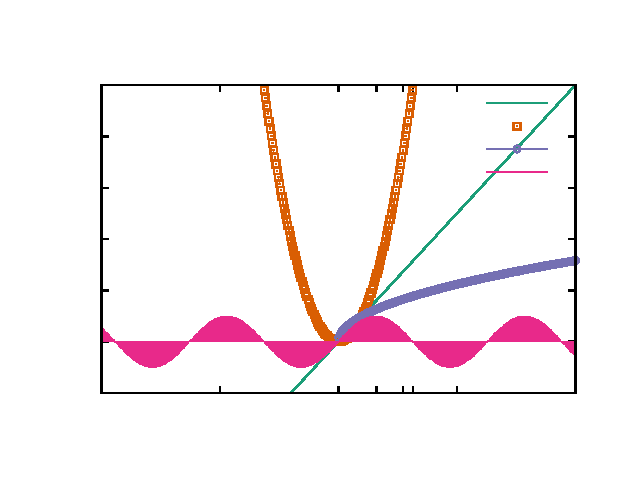
\includegraphics{figures/test/plot}}%
    \gplfronttext
  \end{picture}%
\endgroup
